\documentclass[a4paper,12pt]{article} 

%%% Работа с русским языком
\usepackage{cmap}                           % поиск в PDF
\usepackage{mathtext} 			 	       % русские буквы в формулах
\usepackage[T2A]{fontenc}               % кодировка
\usepackage[utf8]{inputenc}              % кодировка исходного текста
\usepackage[english,russian]{babel}  % локализация и переносы
\usepackage[left=2cm,right=2cm,
    top=2cm,bottom=2cm,bindingoffset=0cm]{geometry}

\usepackage{wrapfig}

\newcommand{\angstrom}{\mbox{\normalfont\AA}} % ангстрем

%Матеша
\usepackage{amsmath,amsfonts,amssymb,amsthm,mathtools, mathrsfs, wasysym}
\usepackage{icomma} % "Умная" запятая

%\mathtoolsset{showonlyrefs=true} % Показывать номера только у тех формул, на которые есть \eqref{} в тексте.

%% Шрифты
\usepackage{euscript}	 % Шрифт Евклид


%%% Заголовок
\author{Гляудялис Гинтарас Б02-104}
\title{Лабораторная работа 4.4.1

Амплитудная дифракционная решетка}
\date{\today}

\begin{document}

\maketitle

\begin{flushleft}
    \hspace*{2.5 mm}
    \textbf{Цели работы:}
    знакомство с работой и настройкой гониометра Г5, 
    определение спектральных характеристик амплитудной 
    решетки. \\
    \hspace*{2.5 mm}
    \textbf{В работе используются:}
    гониометр, дифракционная решетка, ртутная лампа.
\end{flushleft}

\section{Теоретическая часть}
\begin{flushleft}
    \hspace*{2.5 mm}
    Основное соотношение приближенной теории дифракционной решётки:
    \begin{equation}
        d \sin \varphi_m = m \lambda.
    \end{equation}
    \hspace*{2.5 mm}
    Угловая дисперсия $D$ характеризует угловое расстояние между близкими спектральными линиями:
    \begin{equation}
        D = \dfrac{d \varphi}{d \lambda} = \dfrac{m}{d \cos \varphi} = \dfrac{m}{\sqrt{d^2 - m^2 \lambda^2}}.
    \end{equation}
\end{flushleft}

\section{Экспериментальная установка}
\begin{flushleft}
    \hspace*{2.5 mm}
    При работе с дифракционной решёткой основной задачей 
    является точное измерение углов, при которых наблюдаются 
    главные максимумы для различных длин волн. 
    В нашей работе для измерения углов используется 
    гониометр Г5. Принципиальная схема экспериментальной 
    установки приведена на рис. 1. \\
\end{flushleft}

\begin{figure}[h!]
    \centering
    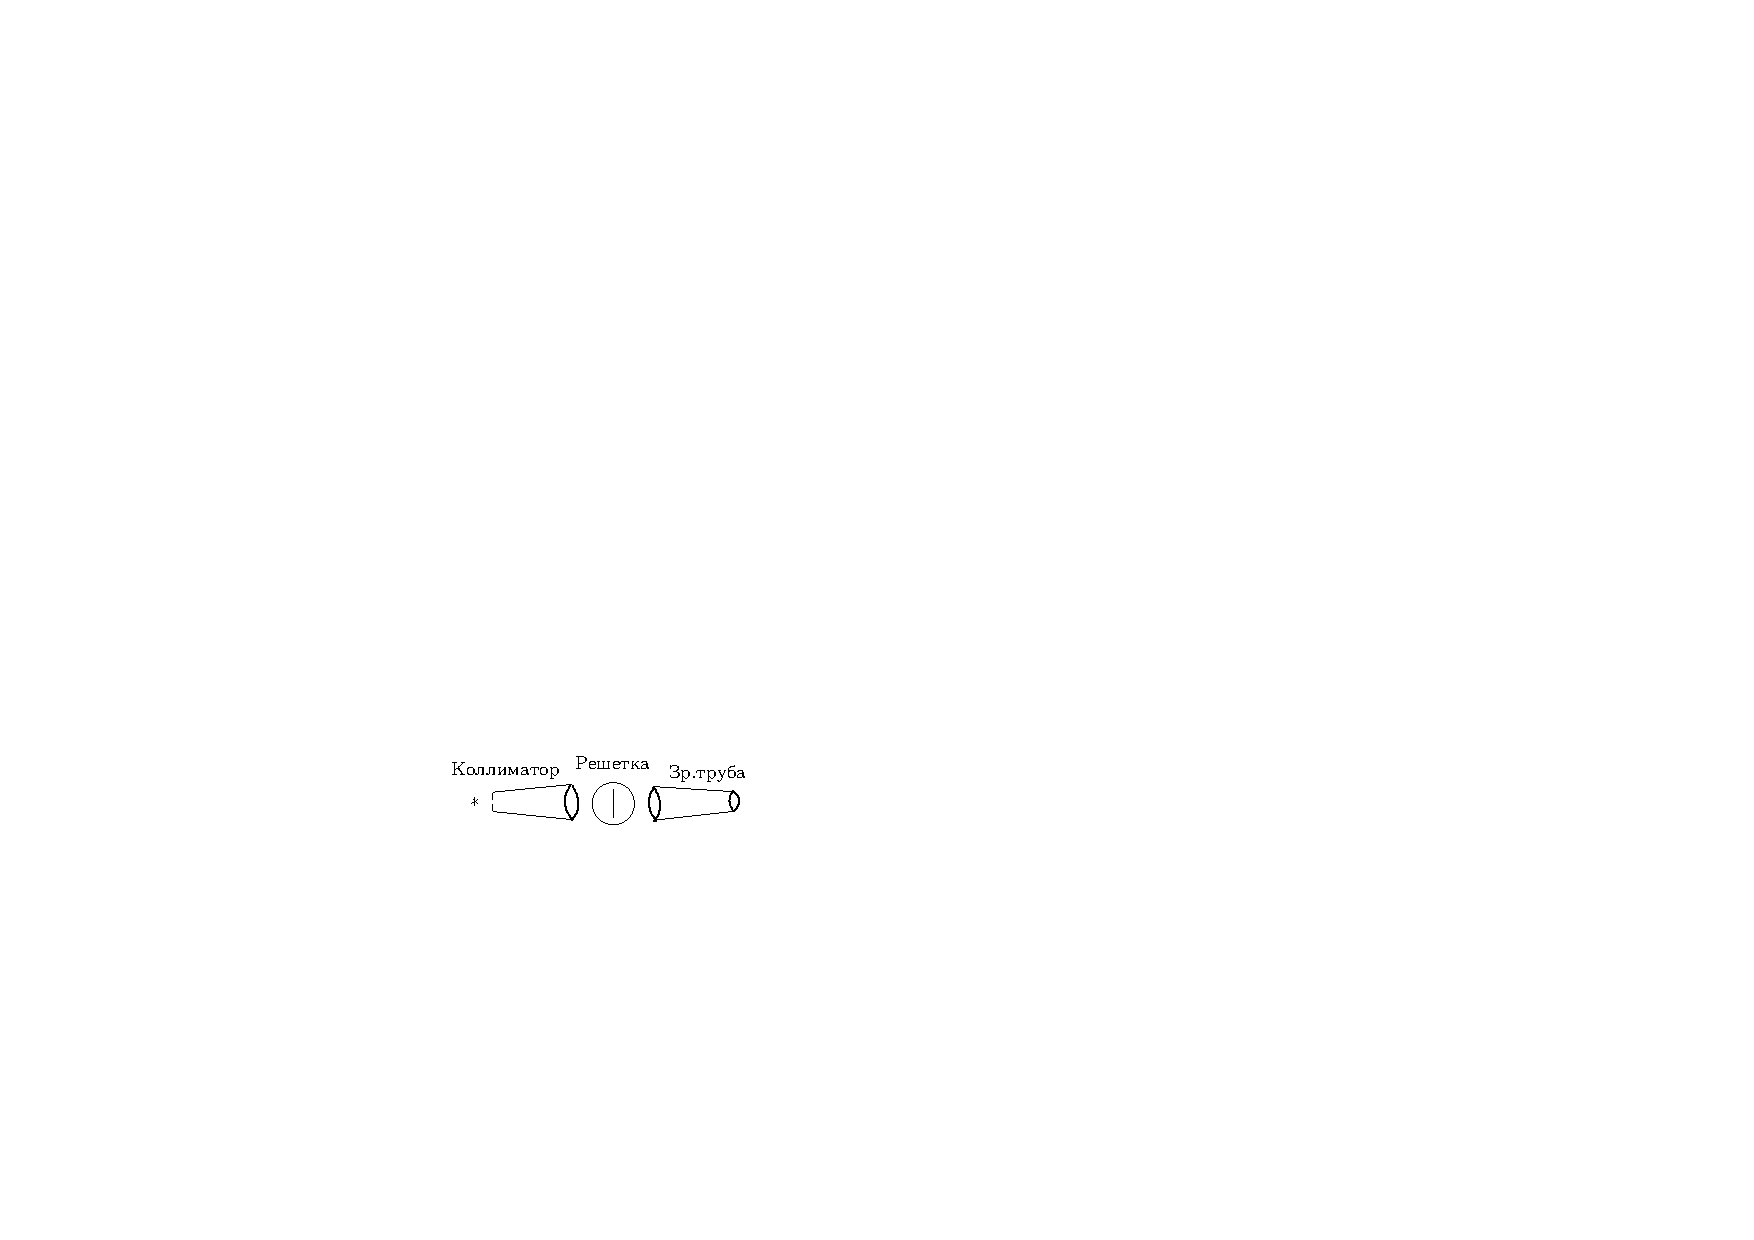
\includegraphics[scale=2]{inst.pdf}
    \caption{Схема установки}
\end{figure}

\section{Экспериментальная часть}
\subsection{Экспериментальные данные}
\begin{flushleft}
    \hspace*{2.5 mm}
    Измерим угловые координаты спектральных линий ртути в $ m = 1 $ 
    порядкеsemithicksemithick, рассчитаем углы дифракции $\varphi_m$. 
    Результаты измерений и вычислений занесем в 
    таблицу~1.
\end{flushleft}

\begin{table}[h!]
    \centering
    \caption{Эксп. данные ($m = 1$)}
    \begin{tabular}{|c|c|c|c|c|c|c|}
        \hline
        $m = 1$ & Синий & Голубой & Зеленый & Желтый (1) & Желтый (2) & Красный \\ \hline
        $\varphi$ & $12 ^{\circ}33'40''$ & $14 ^{\circ}12'19''$ & $15 ^{\circ}48'27''$ & $16 ^{\circ}43'5''$ & $16 ^{\circ}47'41''$ & $18 ^{\circ}6'49''$ \\ \hline
        $\sin \varphi$ & 0.219 & 0.246 & 0.274 & 0.288 & 0.291 & 0.313 \\ \hline
        $\lambda$, нм & 435.8 & 491.6 & 546.1 & 577.0 & 579.1 & 623.4 \\ \hline \hline

        $m = 2$ & Синий & Голубой & Зеленый & Желтый (1) & Желтый (2) & - \\ \hline
        $\varphi$ & $25 ^{\circ}44'37''$ & $29 ^{\circ}19'37''$ & $32 ^{\circ}56'6''$ & $35 ^{\circ}2'36''$ & $35 ^{\circ}11'37''$ & - \\ \hline
        $\sin \varphi$ & 0.436 & 0.491 & 0.544 & 0.575 & 0.578 & - \\ \hline
        $\lambda$, нм & 435.8 & 491.6 & 546.1 & 577 & 579.1 & - \\ \hline
    \end{tabular}
\end{table}

\begin{flushleft}
    \hspace*{2.5 mm}
    Для оценки угловой дисперсии решётки определим разности угловых координат линий жёлтого дублета во всех видимых порядках ($ \Delta \lambda = 21  \angstrom $):
\end{flushleft}

\begin{table}[h!]
    \centering
    \caption{}
    \begin{tabular}{|c|c|c|c|}
        \hline
        $m$ & $\Delta \varphi,~10^{-3}$ рад & $D_{\text{exp}},~10^{-5}~\text{рад}/\angstrom$ & $D_{\text{teor}},~10^{-5}~\text{рад}/\angstrom$ \\ \hline
        1 & 2.91 & 13.9 & 5.0 \\ \hline
        2 & 2.67 & 12.7 & 10.0 \\ \hline
    \end{tabular}
\end{table}

\subsection{Обработка результатов}
\begin{flushleft}
    \hspace*{2.5 mm}
    Построим график зависимости $\lambda (\sin \varphi_m)$ для 1 и 2 порядков:
\end{flushleft}

\begin{figure}[h!]
    \centering
    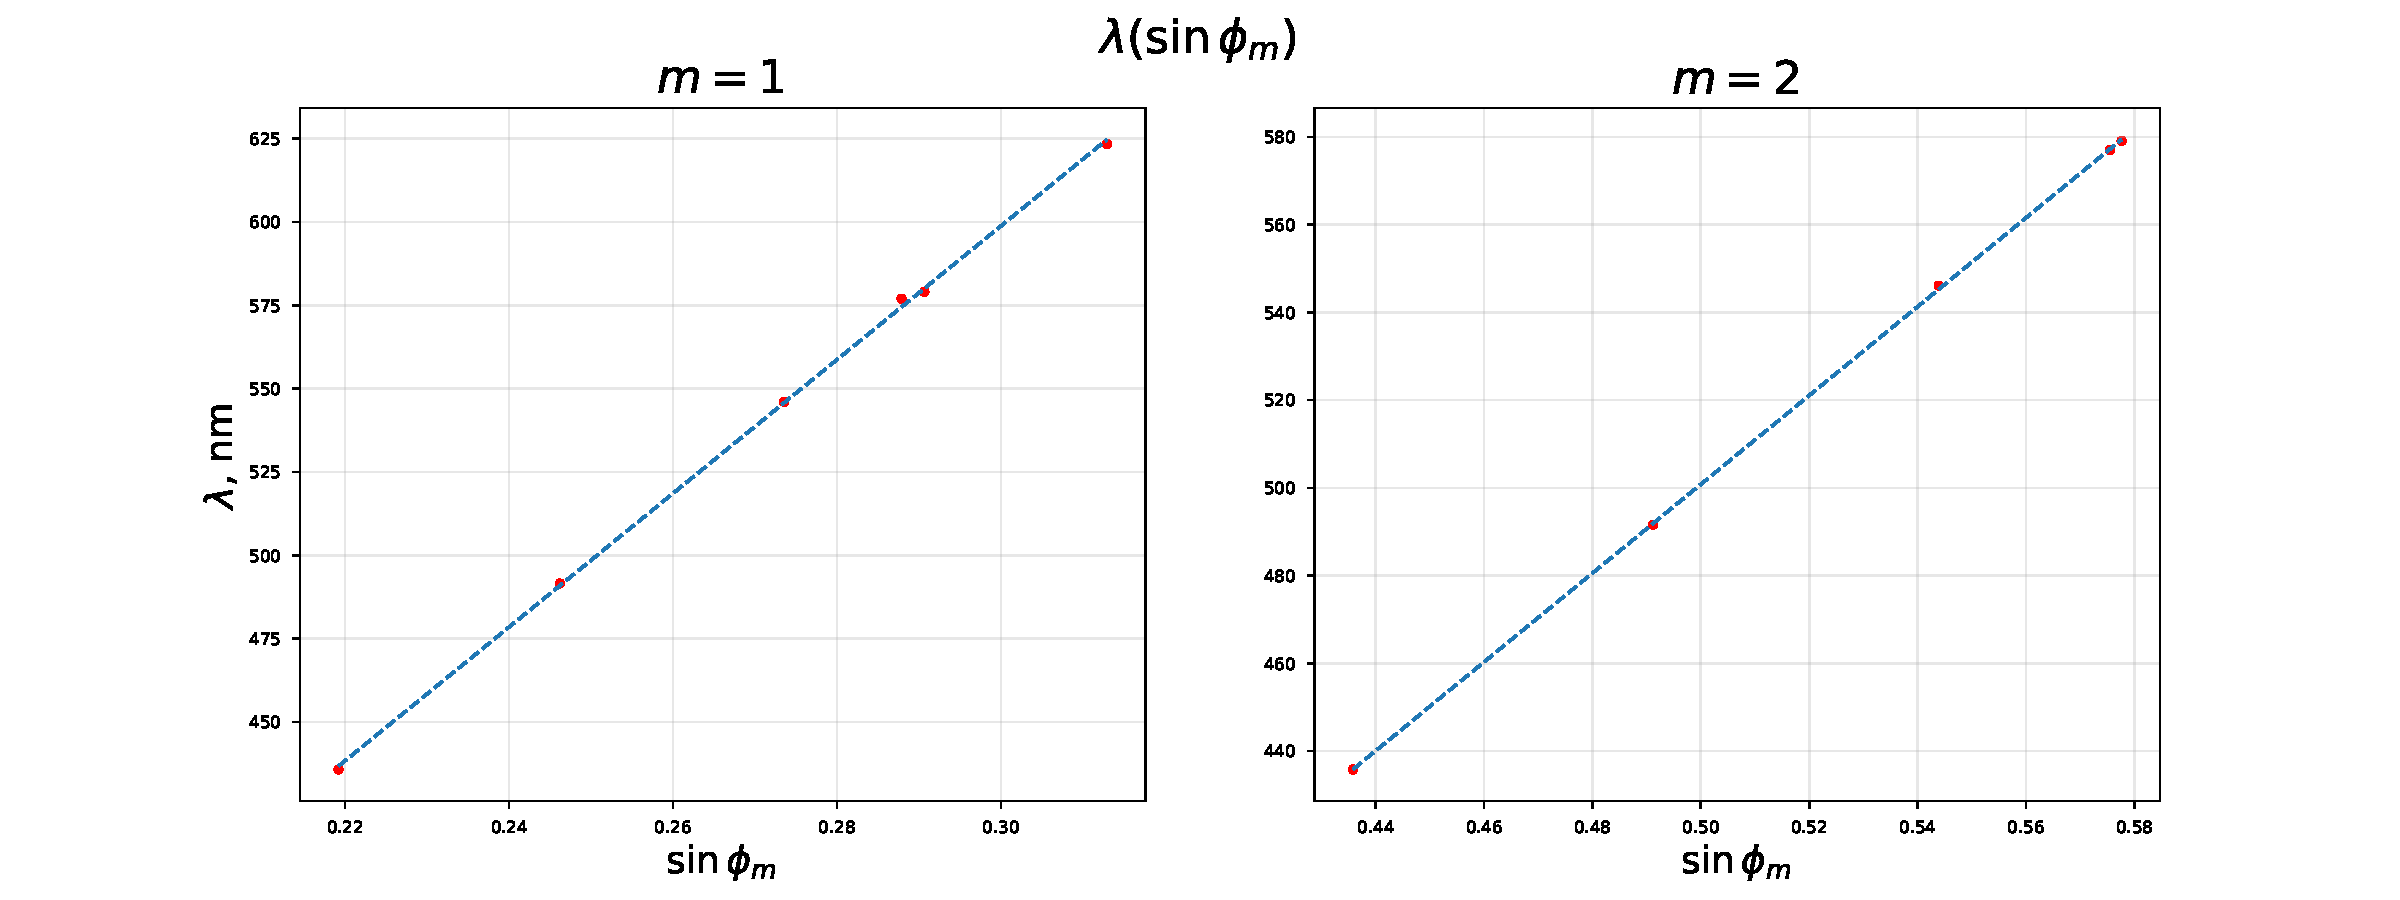
\includegraphics[scale=0.4]{gr.pdf}
    \caption{}
\end{figure}

\begin{flushleft}
    \hspace*{2.5 mm}
    Определим по углу наклона графика период решётки $d$:
    \[d_1 = 2.0 \pm 0.3~\text{мкм},~~d_2 = 2.02 \pm 0.02~\text{мкм}\]
\end{flushleft}

\subsection{Разрешающая способность}

\begin{flushleft}
    \hspace*{2.5 mm}
    Используя формулы
    \[ \delta \lambda \approx \dfrac{d \varphi}{D}, ~~ R \approx \dfrac{\lambda}{\delta \lambda}, ~~ N \approx \dfrac{R}{m}, ~~ l \approx N d \]
    для порядков $m = 1, 2$, получаем
\end{flushleft}

\begin{table}[h!]
    \centering
    \caption{}
    \begin{tabular}{|c|c|c|c|c|}
        \hline
        $m$ & $\delta \lambda,~\angstrom$ & $R$ & $N$ & $l$, мм \\ \hline
        1 & 21.0 & 274.7 & 275 & 0.55 \\ \hline
        2 & 19.2 & 300.5 & 150 & 0.3 \\ \hline
    \end{tabular}
\end{table}

\section{Выводы}

\begin{flushleft}
    \hspace*{2.5 mm}
    Таким образом, мы исследовали спектральные линии ртути, определили шаг решётки, 
    её угловую дисперсию, а также её эффективный размер. Полученные результаты близки 
    к теоретическим вычислениям, за исключением первого порядка.
\end{flushleft}

\end{document}
